
\sloppy
\subsection{Radar application}

The experiments testedin a controlled indoor laboratory environment measuring approximately 6×8 meters. The space included static and dynamic obstacles:

\begin{figure}[H]
    \centering
    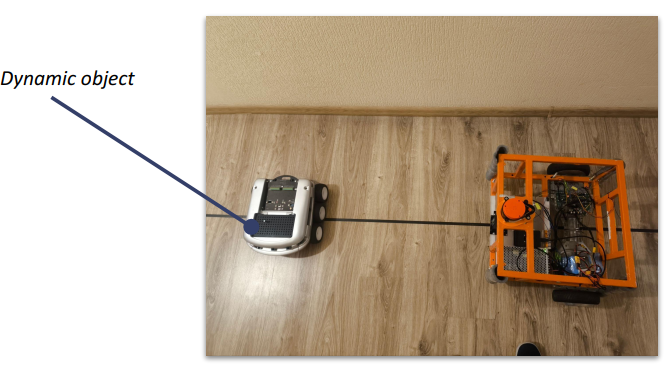
\includegraphics[width=0.5\linewidth]{Src//images/koalarobot.png}
    \caption{Dynamic object on the robot path}
    \label{fig:Objectkoala}
\end{figure}

\begin{itemize}
    \item[\textbf{Static obstacles:}] walls, chairs, talbes, metal objects, metal constructions.
    \item[\textbf{Dynamic obstacles:}] Koala 2.5 robots (see Figure \ref{fig:Objectkoala}) and human operator. Speeds range from $0.2$ to $0.6$ m/s.
    \item[\textbf{Ground truth:}] The speed calculation is determined by the integration of sensors from the encoders of each robot, which facilitate the estimation of the velocity and trajectory of movement. This calculation is further augmented by the incorporation of radar data, thereby enhancing the precision of the measurement.




    
  %  \item[\textbf{Data logging:}] All relevant topics (\texttt{/radar/raw}, \texttt{/radar/points}, \texttt{/odom}, \texttt{/tf}) are recorded using \texttt{ros2 bag} at a frequency of 30 Hz.
\end{itemize}

\subsection{Robot Platform}



\begin{figure}[H]
    \centering
    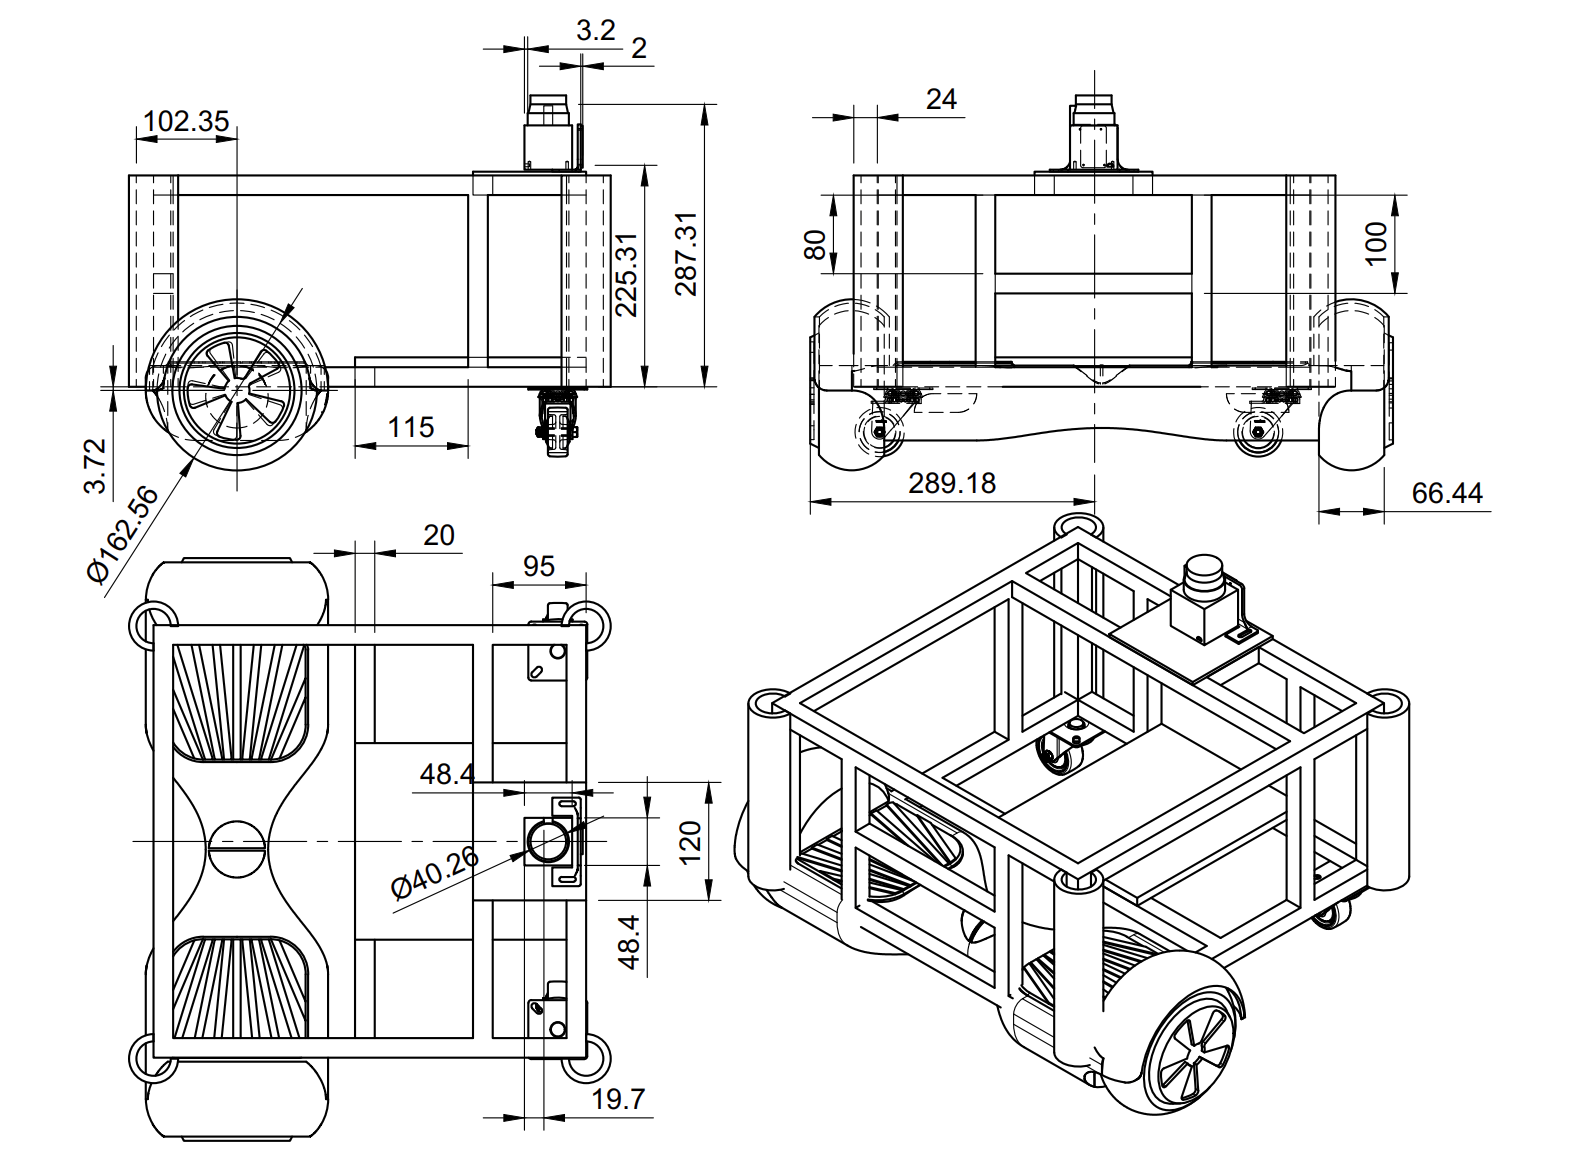
\includegraphics[width=0.6\linewidth]{Src/images/Blackbox.png}
    \caption{Robot platform}
    \label{fig:Robot}
\end{figure}

\begin{itemize}
    \item \textbf{Onboard computer:} Raspberry Pi 4 with 8~GB RAM running Raspberry Pi OS.
    
    \item \textbf{Sensors:}
    \begin{enumerate}
        \item mmWave radar module (60~GHz);
        \item 2D LiDAR Hokuyo URG-04LX-UG01;
        \item Differential wheel odometry with incremental encoders (1024 PPR per wheel).
    \end{enumerate}

    \item \textbf{Mechanical structure:} welded steel chassis (440~mm × 440~mm), 162~mm diameter wheels, BLDC motors with Hall effect sensors (40~V, 120~RPM).
    \item \textbf{Power supply:} 2 × Li-Ion 4S batteries (20~V, 2~Ah) with DC-DC converter (40~V to 5~V).
    \item \textbf{Radar mounting:} radar module fixed on a custom plastic bracket in the front-central zone.
\end{itemize}




\subsection{Kinematic model of mobile platform}
An diy built differential mobile robot is chosen as the carrier
(Fig.~\ref{fig:Differential-model}).
The robot has two independently actuated wheels separated by the
track~\(2L\); the midpoint of the wheel axle is the control
point~\(CP\).\\
In the inertial frame \(OXY\) the robot pose is given by the state vector
\(\boldsymbol{\xi}_r(t)=\bigl[x_r(t),\,y_r(t),\,\theta_r(t)\bigr]^{\mathsf T}\).

\begin{figure}[H]
    \centering
    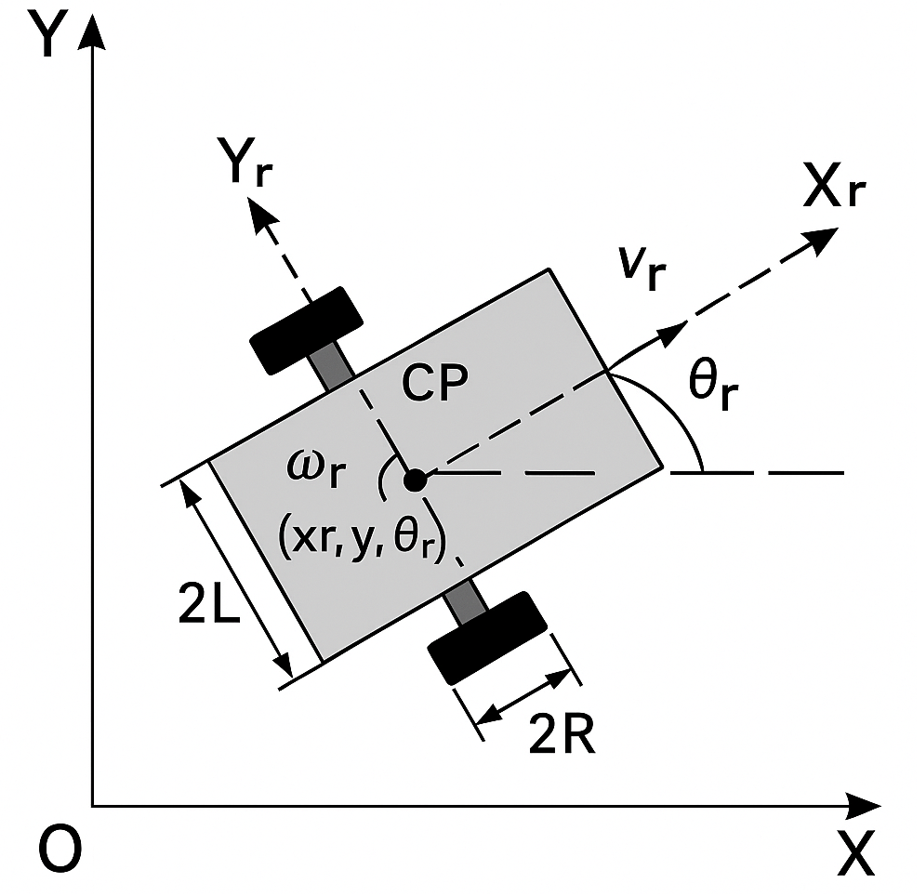
\includegraphics[width=0.5\linewidth]{Src/images/kinematicmodel.png}
    \caption{Differential–drive mobile robot with pose
             \(\bigl(x_r,\,y_r,\,\theta_r\bigr)\)}
    \label{fig:Differential-model}
\end{figure}

Motion is assumed to be \emph{planar} with perfect rolling
(\emph{no slip}).  
Under these assumptions each wheel constrains the velocity of its contact
point to lie along the wheel plane, producing the differential
kinematic model summarised Table \ref{tab:diff_drive_params_en}.
%-----------------------------------------------------------------------------
%-----------------------------------------------------------------------------
\subsubsection{Model Parameters}
\label{sec:model_parameters}

\begin{table}[H]
    \centering
    \caption{Parameters of the Differential-Drive Kinematic Model}
    \label{tab:diff_drive_params_en}
    \begin{tabular}{@{}llll@{}}
        \toprule
        \textbf{Symbol}& \textbf{Typical Value} & \textbf{Unit} & \textbf{Description}  \\
        \midrule
        \(R\)& 0.081 & m & Wheel radius  \\
        \(2L\) & 0.52  & m & Wheel-to-wheel distance (track width)\\
        \(\omega_L,\; \omega_R\) & Up to 20 & rad\,s\(^{-1}\) & Angular speed of left and right wheels \\
        \(v_L,\; v_R\)& Up to 1.6 & m\,s\(^{-1}\)  & Linear speed of left and right wheels \\
        \(v_r\)& Up to 1.6 & m\,s\(^{-1}\) & Linear speed of the robot center  \\
        \(\omega_r\)& Up to 4.0  & rad\,s\(^{-1}\)& Angular velocity (yaw rate) of the robot  \\
        \bottomrule
    \end{tabular}
\end{table}

%-----------------------------------------------------------------------------
\subsubsection{Forward kinematics.}
Equations~\eqref{eq:vr_en}–\eqref{eq:wr_en} map wheel speeds to the
body-frame linear and angular velocity pair \((v_r,\omega_r)\).
The first term in~\eqref{eq:vr_en} represents the \emph{average} wheel
translation, while~\eqref{eq:wr_en} quantifies the \emph{imbalance} between
left and right wheels that produces rotation about the instantaneous centre
of curvature (ICC).  
Because both relations are linear in the wheel rates, they will later be
useful in the design of velocity controllers.

\begin{align}
    v_r      &= \frac{v_R + v_L}{2}
              = \frac{R}{2}\bigl(\omega_R + \omega_L\bigr), \label{eq:vr_en}\\[4pt]
    \omega_r &= \frac{v_R - v_L}{2L}
              = \frac{R}{2L}\bigl(\omega_R - \omega_L\bigr). \label{eq:wr_en}
\end{align}

%-----------------------------------------------------------------------------
\subsubsection{State-space form.}
The compact matrix form~\eqref{eq:diff_drive_matrix} rewrites the nonlinear
kinematics into a drift-free control-affine system, separating the
configuration variables \((x_r,y_r,\theta_r)\) from the control inputs
\((v_r,\omega_r)\).  
This representation is convenient for state-estimation filters
(EKF/UKF/particle-filters) and for the derivation of feedback linearising
controllers.

\begin{equation}
    \dot{\boldsymbol{\xi}}_r =
    \underbrace{%
    \begin{bmatrix}
        \cos\theta_r & 0 \\
        \sin\theta_r & 0 \\
        0            & 1
    \end{bmatrix}}_{\displaystyle B(\theta_r)}
    \begin{bmatrix}
        v_r \\[2pt] \omega_r
    \end{bmatrix},
    \label{eq:diff_drive_matrix}
\end{equation}

\noindent
where \(B(\theta_r)\) is the orientation-dependent input matrix.

Writing~\eqref{eq:diff_drive_matrix} component-wise yields
\begin{subequations}\label{eq:diff_drive_ode_en}
\begin{align}
    \dot{x}_r &= v_r\cos\theta_r, \\
    \dot{y}_r &= v_r\sin\theta_r, \\
    \dot{\theta}_r &= \omega_r.
\end{align}
\end{subequations}

%-----------------------------------------------------------------------------
\subsubsection{Inverse kinematics}
For motion planning or trajectory-tracking the required wheel rates can be
computed from the desired body velocities
\(\bigl(v_r^\ast,\omega_r^\ast\bigr)\) by rearranging
Eqs.~\eqref{eq:vr_en}–\eqref{eq:wr_en}:

\begin{align}
    \omega_L &= \frac{v_r^\ast - L\,\omega_r^\ast}{R}, &
    \omega_R &= \frac{v_r^\ast + L\,\omega_r^\ast}{R}.
    \label{eq:inverse_kinematics_en}
\end{align}

\noindent
The expressions in~\eqref{eq:inverse_kinematics_en} emphasise that turning
(\(\omega_r^\ast \neq 0\)) is achieved by introducing a differential speed
between the wheels, whereas pure translation
(\(\omega_r^\ast = 0\)) requires identical wheel rates.

%-----------------------------------------------------------------------------
\subsubsection{Pose integration}
For digital implementation the continuous-time model was integrated.
Using a simple forward Euler rule over the sampling period \(\Delta t\)
gives

\begin{equation}
    \boldsymbol{\xi}_r(k+1)=
    \begin{bmatrix}
        x_r(k) + v_r(k)\cos\theta_r(k)\,\Delta t \\
        y_r(k) + v_r(k)\sin\theta_r(k)\,\Delta t \\
        \theta_r(k) + \omega_r(k)\,\Delta t
    \end{bmatrix}.
    \label{eq:euler_update}
\end{equation}


\subsubsection{Encoder and timing parameters}

Incremental quadrature encoders mounted on the robot's driving wheels are used to estimate the robot's displacement. Each encoder produces \(N_\text{ppr}\) pulses per full rotation of the wheel. \(\Delta N_L,\;\Delta N_R\) denote the number of pulses received from the left and right encoders during a sampling interval \(\Delta t\).

\paragraph{Angular displacement of wheels.}
The angular displacement for each wheel can be calculated as:
\begin{equation}
    \Delta\varphi_L = \frac{2\pi\,\Delta N_L}{N_\text{ppr}},\qquad
    \Delta\varphi_R = \frac{2\pi\,\Delta N_R}{N_\text{ppr}}.
    \label{eq:wheel_angle_inc}
\end{equation}
Here, \(N_\text{ppr}\) is the number of pulses per revolution (PPR) of the encoder.

\paragraph{Linear displacement of wheels.}
Using the wheel radius \(R\), the linear travel of each wheel is:
\begin{equation}
    \Delta s_L = R\,\Delta\varphi_L,\qquad
    \Delta s_R = R\,\Delta\varphi_R.
\end{equation}

\paragraph{Incremental odometry model.}
Assuming small angular changes, the robot’s orientation increment is given by:
 $
    \Delta\theta_r = \frac{\Delta s_R - \Delta s_L}{2L},
 $
where \(2L\) is the distance between the wheels (wheelbase). The robot's pose \((x_r, y_r, \theta_r)\) is then updated:
\begin{align}
    x_r^{k+1} &= x_r^{k} + \frac{\Delta s_L + \Delta s_R}{2}\,
                \cos\!\left(\theta_r^{k} + \frac{\Delta\theta_r}{2}\right),\\[2pt]
    y_r^{k+1} &= y_r^{k} + \frac{\Delta s_L + \Delta s_R}{2}\,
                \sin\!\left(\theta_r^{k} + \frac{\Delta\theta_r}{2}\right),\\[2pt]
    \theta_r^{k+1} &= \theta_r^{k} + \Delta\theta_r.
    \label{eq:odom_update}
\end{align}
This method assumes constant velocity during \(\Delta t\) and performs an arc-based motion update.



% \begin{table}[H]
%     \centering
%     \caption{Encoder specifications and odometry update timing}
%     \label{tab:encoder_params}
%     \begin{tabular}{@{}llp{6.2cm}@{}}
%         \toprule
%         \textbf{Parameter} & \textbf{Value} & \textbf{Description} \\ \midrule
%         Encoder resolution, \(N_\text{ppr}\) & 2048~imp/rev &
%             Total number of pulses per revolution, including quadrature encoding. \\
%         Sampling interval, \(\Delta t\) & 10~ms &
%             Odometry update cycle (ROS~2 timer or real-time loop). \\
%         Max wheel speed, \(\omega_{\max}\) & 20~rad/s &
%             Limited by motor driver or safety software. \\
%         Max displacement per \(\Delta t\) &
%             \(R\,\omega_{\max}\Delta t\) &
%             Useful to detect possible encoder errors or wheel slip. \\
%         \bottomrule
%     \end{tabular}
% \end{table}






\subsection{Tasks and scenarios}

During testing, a mobile platform was used, which is shown in the Figure \ref{fig:platform}.


\begin{figure}
    \centering
    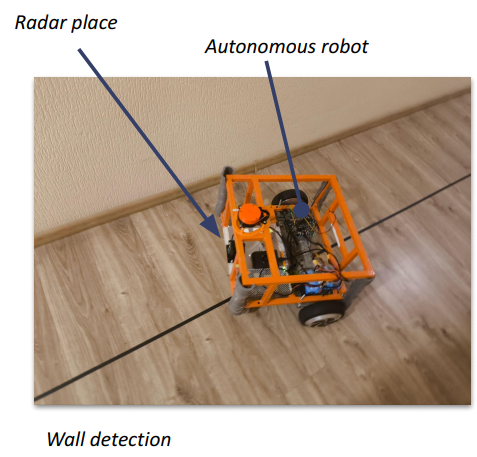
\includegraphics[width=0.5\linewidth]{Src//images/Robot.png}
    \caption{Robot platform}
    \label{fig:platform}
\end{figure}


\subsection{Architecture of the motion planning system}
The motion planning system leverages the Robot Operating System 2 (ROS2) framework, chosen for its modularity, real-time capabilities, and extensive libraries for robotic applications.
\begin{figure}[H]
    \centering
    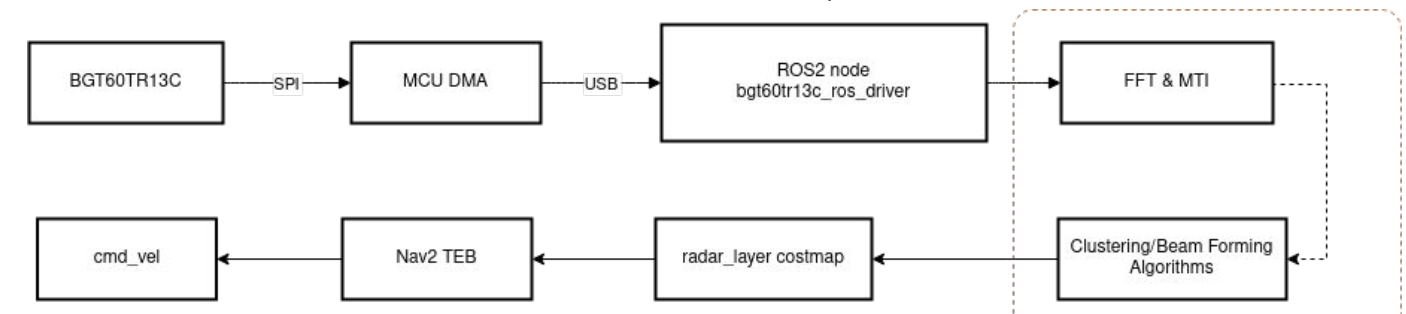
\includegraphics[width=1\linewidth]{Src/images/Algorthm.png}
    \caption{Radar ROS data path flow}
    \label{fig:radar_ros}
\end{figure}
\begin{itemize}
    \item \textbf{Radar Data Acquisition:} The BGT60TR13C radar initiates an FMCW ramp. The MCU on the radar board reads the I/Q signals from the three receivers via SPI and transmits this raw data, often via USB, to the host computer Raspberry Pi 4 on the robot platform.
    \item \textbf{Signal Processing Pipeline:} On the host, a series of ROS2 nodes process the raw data. This includes FFT for range information, MTI to distinguish moving targets, and Digital Beamforming (DBF) for angle estimation
    \item \textbf{Target Tracking and Publication:} Detected targets (with position and velocity) are published to a dedicated ROS2 topic \textit{/radar/tracks}
    \item \textbf{Costmap Integration:} A custom radar\_layer plugin subscribes to \textit{/radar/tracks} and updates the local costmap within the Nav2 stack. Obstacles detected by the radar are inserted into this costmap
    \item Path Planning and Execution: The Nav2 navigation stack re-plans the robot's path based on the updated costmap, generating cmd\_vel commands to control the robot's motors and navigate around obstacles
\end{itemize}
\subsubsection{Software architecture}

The software architecture is built upon several ROS2 packages avalable in Appendix 1, each handling specific functionalities:
\begin{itemize}
    \item \textbf{\texttt{bgt60\_driver}}: This package contains the primary node for interfacing with the BGT60TR13C radar.
    \begin{itemize}
        \item \textbf{Node}: \texttt{bgt60tr13c\_ros\_driver}.
        \item \textbf{Functionality}: Handles communication with the radar hardware via the Atmel MCU on the demo board, acquires raw data from the antennas, and manages radar configuration parameters. It publishes to \texttt{/bgt60/iq\_raw} and temperature data to \texttt{/bgt60/temp}.
    \end{itemize}
    \item \textbf{\texttt{radar\_dsp} (Digital Signal Processing)}: This package is responsible for the initial processing of the raw radar signals.
    \begin{itemize}
        \item \textbf{Node(s)}: May consist of one or more nodes for sequential processing.
        \item \textbf{Functionality}: Subscribes to \texttt{/bgt60/iq\_raw}. Performs Fast Fourier Transform (FFT) to extract range information and Moving Target Indication (MTI) to filter out static clutter and highlight dynamic objects. Noise compensation techniques may also be applied here.
    \end{itemize}
    \item \textbf{\texttt{radar\_tracker}}: This package focuses on higher-level object processing.
    \begin{itemize}
        \item \textbf{Node(s)}: A dedicated node for object detection, clustering, and tracking.
        \item \textbf{Functionality}: Subscribes to \texttt{/bgt60/detections}. Implements algorithms for Digital Beamforming (DBF) to estimate the angle of detected targets which are published to \texttt{/radar/tracks}.
    \end{itemize}
    \item \textbf{\texttt{radar\_layer}}: This package integrates the radar data into the Nav2 navigation stack.
    \begin{itemize}
        \item \textbf{Plugin}: A custom costmap layer plugin for Nav2.
        \item \textbf{Functionality}: Subscribes to \texttt{/radar/tracks}. Updates the local cost map by marking cells corresponding to the positions of the detected obstacles, allowing Nav2 to account for them during path planning. This is crucial for adapting the robot's trajectory based on mmWave radar data.
    \end{itemize}
    \item \textbf{\texttt{nav2\_bt\_navigator} \& Core Nav2 Packages}: These standard Nav2 components handle the overall navigation logic.
    \begin{itemize}
        \item \textbf{Functionality}: The Behavior Tree navigator orchestrates high-level navigation tasks, switching between behaviors like 'drive' or 'dodge' based on the costmap information. Planners the TEB (Timed Elastic Band) local planner utilize the radar-updated costmap to generate collision-free \texttt{cmd\_vel} commands.
    \end{itemize}
    \item \textbf{Diagnostics}: A \texttt{diagnostics\_agg} topic aggregates status messages from the radar system, such as operating temperature or SPI communication integrity, crucial for system monitoring.
    

\subsubsection{Algorithm implementation}

The transformation of raw radar data into actionable information for motion planning involves several key algorithmic steps, building upon the experiments detailed in Chapter 3:

\begin{enumerate}
    \item \textbf{Raw Data Ingestion and Framing}: The \texttt{bgt60\_driver} node acquires raw I/Q samples for each chirp across the three RX antennas. This data is structured into frames, as described by the "Raw Data representing" cube Figure 3.9.
    \item \textbf{Range Profile Generation (1D FFT)}: For each chirp and each antenna, a 1D FFT is applied to the time-domain I/Q samples. The magnitude of this FFT output provides a range profile, where peaks indicate the presence of objects at corresponding distancesEquation 7 and Equation 8. This was experimentally validated in section 3.4.1.
    \item \textbf{Clutter Reduction (Mean Removal \& MTI)}:
    \begin{itemize}
        \item \textbf{Mean Removal}: The DC component from each chirp signal is removed by subtracting the chirp-wise average Equation 9.
        \item \textbf{Moving Target Indication (MTI)}: To suppress static clutter (reflections from walls, stationary furniture) and moving targets, a high-pass filter is applied along the slow-time (inter-chirp) axis Equation 10 . The effectiveness of MTI was demonstrated in the environmental noise tests Figure 3.12and the "animal detection" experiment Figure 3.15.
    \end{itemize}
    \item \textbf{Amplitude Cutoff}: To further reduce noise and retain significant detections, a threshold is applied to the MTI-filtered data, setting values below -60 dB relative to the peak to zero.
    \item \textbf{Range-Doppler Map Generation (2D FFT)}: A second FFT is performed across the chirps within a frame (slow-time) for each range bin. This generates a Range-Doppler map, where signal energy peaks indicate both the range and radial velocity of targets. This is fundamental for determining object velocity.
    \item \textbf{Direction-of-Arrival (DoA) Estimation (DBF)}: Using the data from the multiple RX antennas, Digital Beamforming (DBF) techniques are employed to estimate the angle of arrival (AoA) of the signals. The Range-Angle 2D DBF method, as described in section 3.4.3, applies a spatial FFT across the antenna channels for each significant range bin to construct a 2D range-angle map Figure 3.16. This allows for localization of targets in the angular domain. The BGT60TR13C's L-shaped arrangement of three antennas enables both azimuth and some vertical direction detection.
    \item \textbf{Costmap Update}: The \texttt{radar\_layer} node subscribes to these tracked objects. It translates their estimated positions (and potentially predicted future positions based on velocity) into the robot's 2D coordinate frame and updates the Nav2 local costmap by marking the corresponding cells as occupied or inflated. This directly feeds information about dynamic obstacles into the robot's path planner.
\end{enumerate}

The behavior tree depicted in Figure~\ref{fig:BT_Navigator} is particularly well-suited for situations where a mobile robot must autonomously navigate to a target location in an environment shared with other robots. A typical example is a warehouse setting, where multiple robots operate in confined spaces such as narrow aisles, which can lead to frequent and unpredictable dynamic obstacles.

\end{itemize}
\begin{figure}[H]
    \centering
    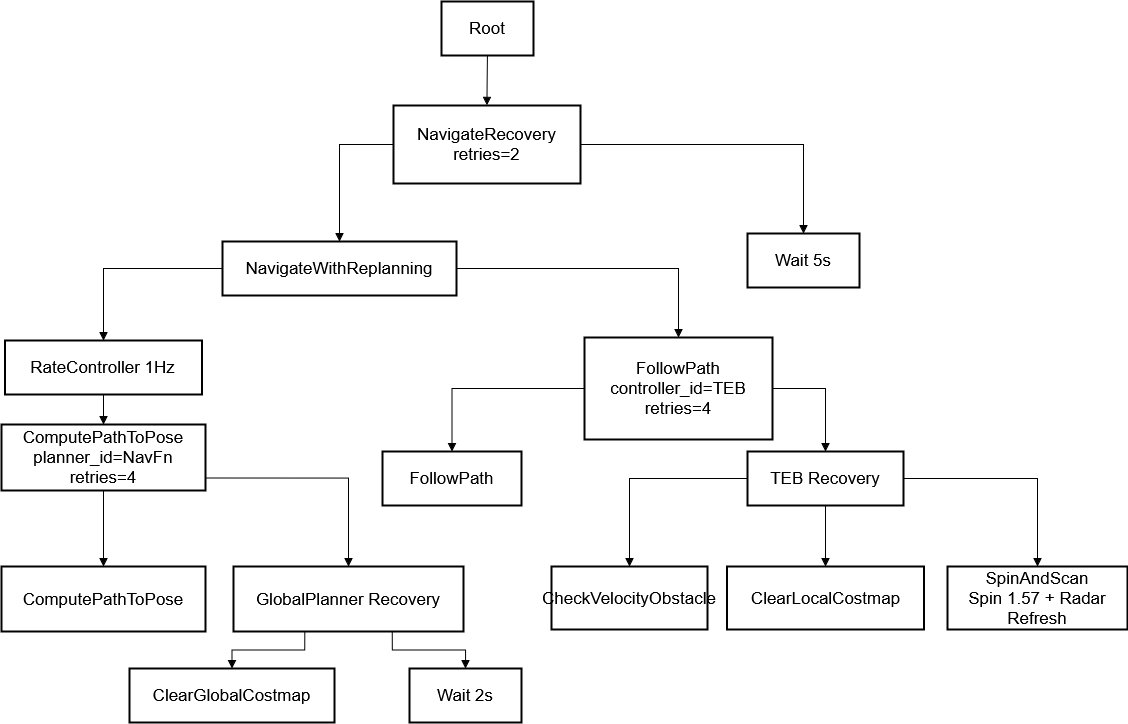
\includegraphics[width=\linewidth]{Src//images/bt.png}
    \caption{BT Navigator tree}
    \label{fig:BT_Navigator}
\end{figure}


The navigation process starts with the \texttt{NavigateWithReplanning} node, which continuously updates the global path in response to changes in the environment. If another robot blocks the planned route, the system detects this during the \texttt{FollowPath} stage. If the robot fails to progress repeatedly, the behavior tree triggers the \texttt{Planner Recovery} subtree: the robot clears its local costmap using \texttt{ClearLocalCostmap} and performs a local rotation (\texttt{Spin 1.57} rad) to refresh its local perception.
Simultaneously, if the global path calculation fails, such as when both robots remain stationary while waiting for the other to move, the ComputePathToPose node activates its own recovery process. This process includes clearing the global costmap and pausing for a short period (Wait 2s) to allow surrounding agents to proceed, potentially resolving the mutual obstruction.
If all attempts at recovery fail, the Wait 5s node is triggered as a final fallback. This pause allows for additional time for environmental changes to occur, such as the opposing robot completing its trajectory, thereby resolving the deadlock without the need for explicit communication between agents.
This layered and responsive structure ensures reliable navigation in multi-agent environments, promoting decentralized coordination and minimizing the reliance on centralized control mechanisms.


\subsubsection{Algorithm for Obstacle Avoidance in Corridors}

\begin{figure}[H]
    \centering
    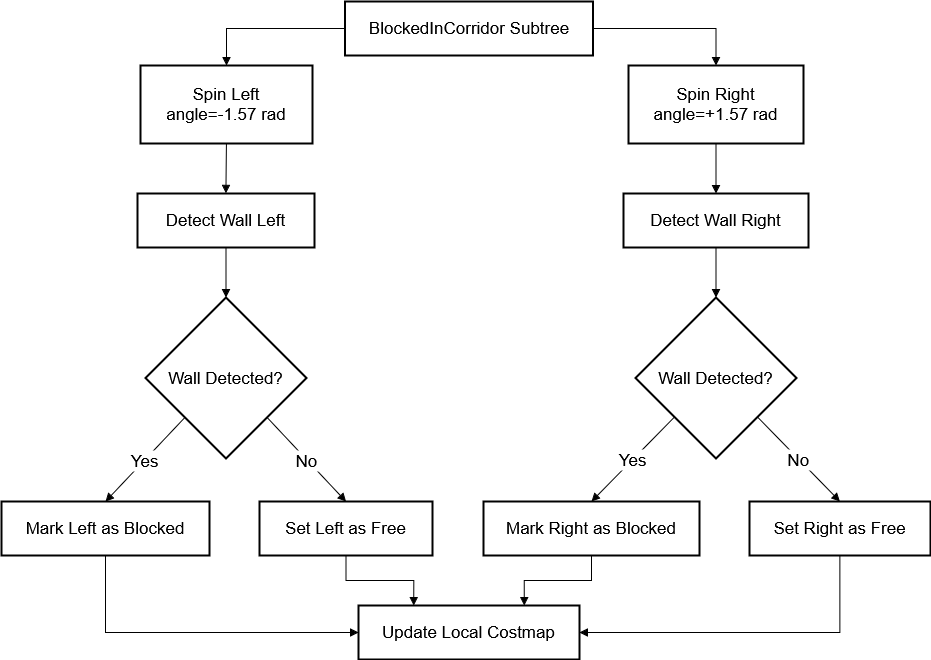
\includegraphics[width=0.8\linewidth]{Src//images/bttreecorodor.png}
    \caption{Subtree for obstacle avoidance in narrow corridor}
    \label{fig:bt_corridor}
\end{figure}

In constrained environments such as narrow corridors, traditional path following may fail due to sudden blockages. The presented Behavior Tree subtree (Figure ~\ref{fig:bt_corridor}) outlines a local reactive strategy that enables the robot to assess both sides before attempting further movement. 

Upon detecting a blockage, the robot first rotates to the left (\(-90^\circ\)) and scans for nearby walls using onboard sensors. If a wall is detected, the left direction is marked as blocked in the local map. The robot then repeats the procedure to the right (\(+90^\circ\)). Based on the results of both checks, the local costmap is updated, enabling informed replanning. This behavior ensures spatial awareness in tight environments and minimizes the risk of deadlock.


\subsubsection{Algorithm for Many Obstacles}
When multiple obstacles are detected along the planned path, the robot requires more complex decision-making to maintain safe and efficient navigation. The Behavior Tree presented in Figure~\ref{fig:bt_multi_obstacle} illustrates a reactive obstacle-handling strategy that adapts based on both the number and type of detected objects.

\begin{figure}[H]
    \centering
    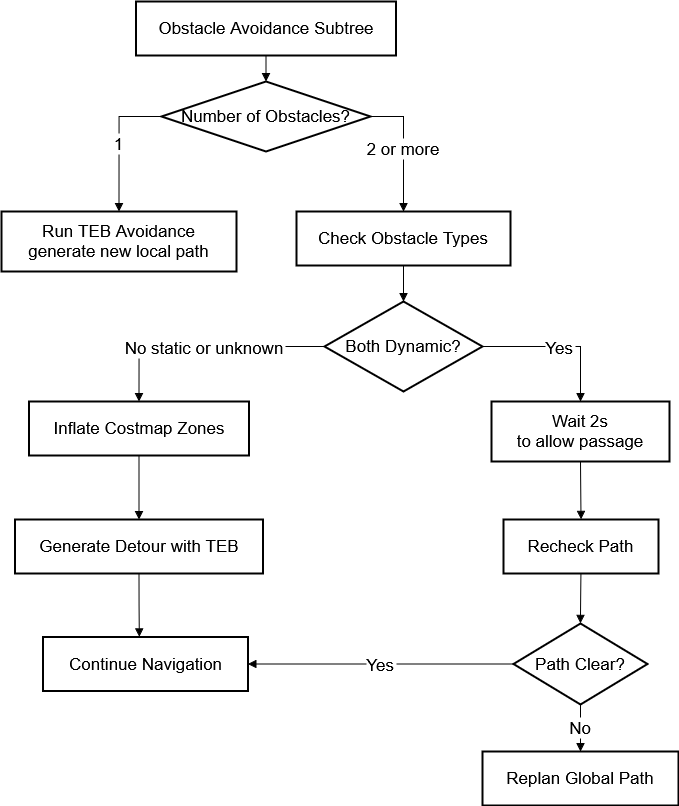
\includegraphics[width=0.65\linewidth]{Src//images/2obstaclebt.png}
    \caption{Behavior Tree subtree for handling multiple obstacles on the path}
    \label{fig:bt_multi_obstacle}
\end{figure}



The robot first identifies the obstacles and estimates their count and behavior using radar with LiDAR. If a single obstacle is detected, a local path is generated using the TEB (Timed Elastic Band) planner to avoid it. In the case of two or more obstacles, the robot performs a type check: if all detected objects are dynamic ( humans or moving robots), it temporarily pauses to allow them to pass and then re-evaluates the path. If the objects are static or unclassified, the robot inflates their costmap areas and attempts to find a detour using local replanning.

\subsection{Experimental results}

This section will present the quantitative and qualitative results from the experiments conducted to evaluate the of the mmWave radar-based motion planning system. The evaluation will focus on the system's ability to reliably detect obstacles, estimate their properties (range, velocity, angle), and enable the robot to navigate in the described dynamic indoor scenarios.


\subsubsection{Static Obstacle Detection and Ranging}
\begin{itemize}
    \item \textbf{Methodology}:  
    The robot performs static obstacle detection experiments in an indoor environment using its radar sensor. When a stationary object is detected (a wall or a box) and there is insufficient free space for maneuvering, the robot enters a passive wait mode (\texttt{Wait 2s}). If the obstacle remains, it performs an in-place rotation to reevaluate its surroundings before replanning. Ground-truth distances were measured manually or with a calibrated LiDAR for comparison.

    \item \textbf{Metrics}:
    \begin{itemize}
        \item Mean Absolute Error (MAE) and Root Mean Square Error (RMSE) between radar-measured and ground-truth distances.
        \item Number of successful recovery rotations when no local path was available.
    \end{itemize}

    \item \textbf{Expected Visualizations}:
    \begin{itemize}
        \item Scatter plots of radar-estimated vs actual distances, including error bars.
    \end{itemize}
\end{itemize}

\begin{table}[H]
\centering
\caption{Radar-based distance estimation vs. ground truth for static obstacles}
\begin{tabular}{@{}lcccc@{}}
\toprule
\textbf{Object Type} & \textbf{Material} & \textbf{True Distance (m)} & \textbf{Radar Estimate (m)} & \textbf{Abs. Error (m)} \\
\midrule
Wall corner         & Concrete  & 1.00 & 0.90 & 0.10 \\
Cardboard box       & Cardboard & 1.20 & 0 & 1.20 \\
Metal cabinet       & Steel     & 1.50 & 1.49 & 0.01 \\
Wooden shelf        & Wood      & 1.80 & 1.86 & 0.06 \\
Water container     & Plastic/water & 2.00 & 1.95 & 0.05 \\
\bottomrule
\end{tabular}
\label{tab:radar_accuracy}
\end{table}
\begin{figure}[H]
    \centering
    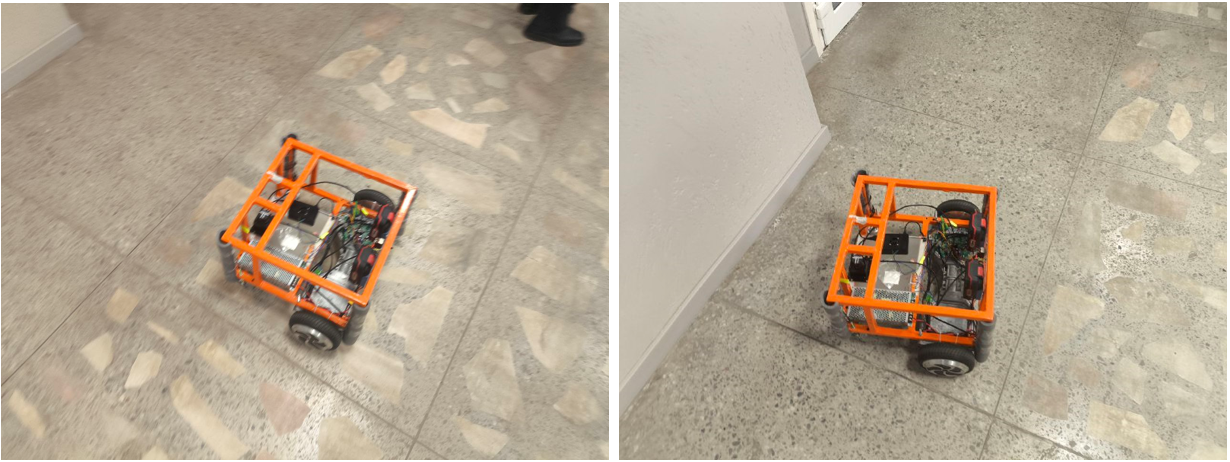
\includegraphics[width=1\linewidth]{Src//images/robotWall.png}
    \caption{Robot and  wall detection}
    \label{fig:Robotwall}
\end{figure}
\noindent
Table~\ref{tab:radar_accuracy} shows that radar achieves sub-\SI{10}{cm} accuracy in most cases.  
In test runs where the robot faced an impassable obstacle, it waited for \SI{2}{s} before initiating a recovery rotation.



\begin{figure}[H]
    \centering

     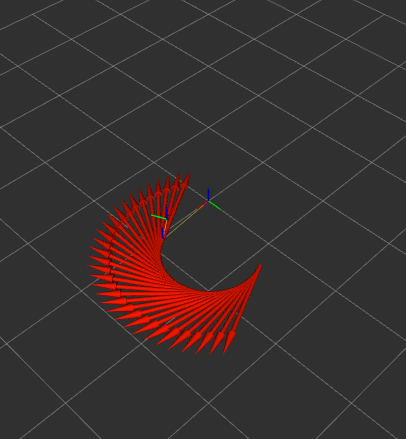
\includegraphics[width=0.3\linewidth]{Untitled.png}
    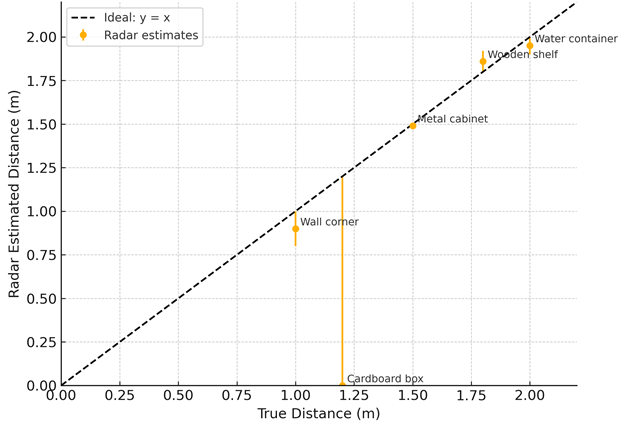
\includegraphics[width=0.48\linewidth]{Src//images/scatterplot.png}
    \caption{ Left: Rviz path planning Right:Scatter plot with error bars}
    \label{fig:Scatter}
\end{figure}

\subsubsection{Navigation Performance and Obstacle Avoidance}
\begin{itemize}
    \item \textbf{Methodology}: End-to-end tests where the robot navigates a predefined path or to a goal point in the presence of static and dynamic obstacles.
    \item \textbf{Metrics}:
    \begin{itemize}
        \item Success rate of task completion (reaching goal without collision).
        \item Number of collisions or near-misses.
        \item Path (path length, time taken) compared to an obstacle-free run or LIDAR-based navigation.
        \item Smoothness of trajectory adjustments.
    \end{itemize}
    \item \textbf{Expected Visualizations}:
    \begin{itemize}
        \item Robot trajectories plotted on a map of the environment, showing avoidance maneuvers.
        \item Videos of the robot successfully navigating challenging scenarios.
        \item Comparison of costmap updates generated by the radar layer versus a LIDAR-based layer if available.
    \end{itemize}
\end{itemize}

\begin{figure}[H]
    \centering
    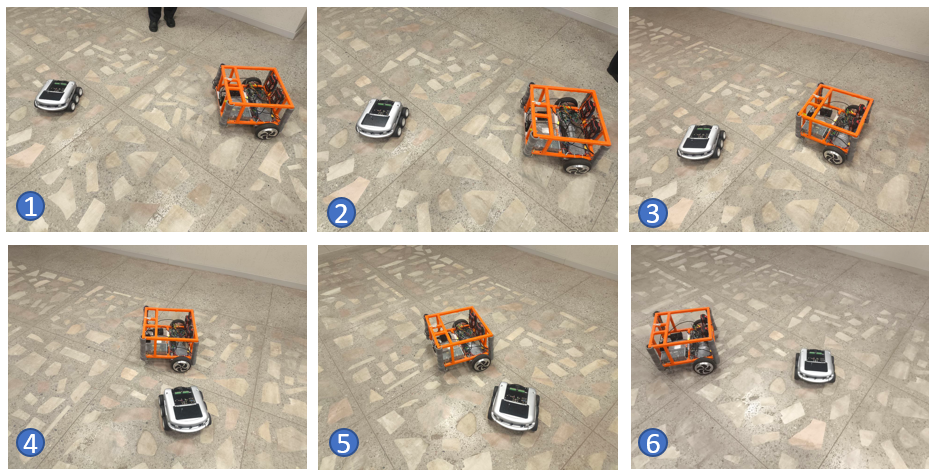
\includegraphics[width=1\linewidth]{Src//images/object.png}
    \caption{Obstacle avoidance}
    \label{fig:enter-label}
\end{figure}


\paragraph{(a) Visual overview.}
Frames~1–6 depict the white delivery robot meeting an orange inspection robot.
After detecting the moving obstacle, the delivery robot initiates its avoidance manoeuvre,
executes a lateral diversion, and finally realigns with the original global path.

\begin{figure}[H]
    \centering
    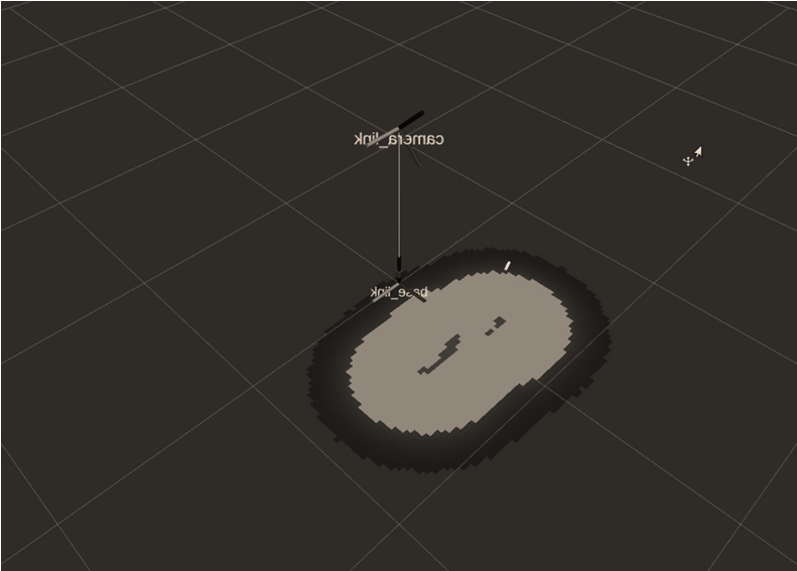
\includegraphics[width=0.5\linewidth]{Src//images/Ros2Obstacle.png}
    \caption{Rviz2 Obstacle data representrative}
    \label{fig:Rviz2_Obstacle}
\end{figure}

The cyan cost map 2d represents raw detections fused from mmWave.
Concentric costmap rings (blue–purple) indicate inflated obstacle layers used by the local planner.
The robot footprint and heading are shown by the green arrow.


\begin{figure}[H]
    \centering
    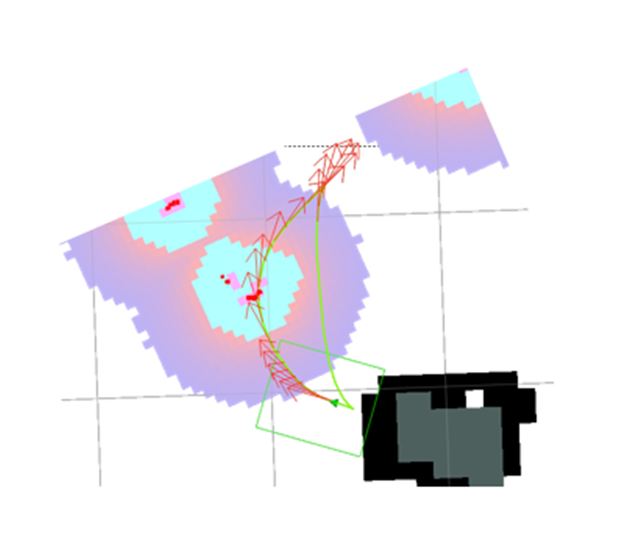
\includegraphics[width=0.5\linewidth]{Src/images/image(18).PNG}
    \caption{TEB path Planing}
    \label{fig:TEB}
\end{figure}


Using the costmap \ref{fig:Rviz2_Obstacle} in, the TEB algorithm generates the yellow, time-parameterised trajectory On Figure \ref{fig:TEB} that bends around the inflated region while satisfying the robot’s kinematic constraints.
Red ellipses outline the dynamically updated obstacle hulls; the shaded cyan footprint confirms that no
part of the path violates safety margins.

This combined view demonstrates the closed loop of perception, costmap generation, and local
optimization: Sensor data are converted into a spatial cost representation, and TEB continuously replans a
collision-free path, enabling reliable navigation in the presence of other autonomous agents.